This section demonstrate the phase-transition phenomenon in model \eqref{eq:model-chisq} with numerical experiments.

The sparsity and signal size of the sparse mean vector are parametrized as in Theorem \ref{thm:chi-squred-strong-boundary}.

\subsection{The strong classification boundary in finite dimensions}

The support set $S$ is estimated using Bonferroni's procedures with FWER decreasing at a rate of $1/\sqrt{\log{p}}$, therefore satisfying the assumptions in Theorem \ref{thm:chi-squred-strong-boundary}.
Experiments were repeated 1000 times under each sparsity-and-signal-size combination.

The results of the numerical experiments are shown in Figure \ref{fig:phase-simulated-chi-squared}.
The numerical results illustrate that the predicted boundaries are not only accurate in high-dimensions ($p=10000$, right panels of Figure \ref{fig:phase-simulated-chi-squared}), but also practically meaningful even at moderate dimensions ($p=100$, left panels of Figure \ref{fig:phase-simulated-chi-squared}).


\begin{figure}
      \centering
      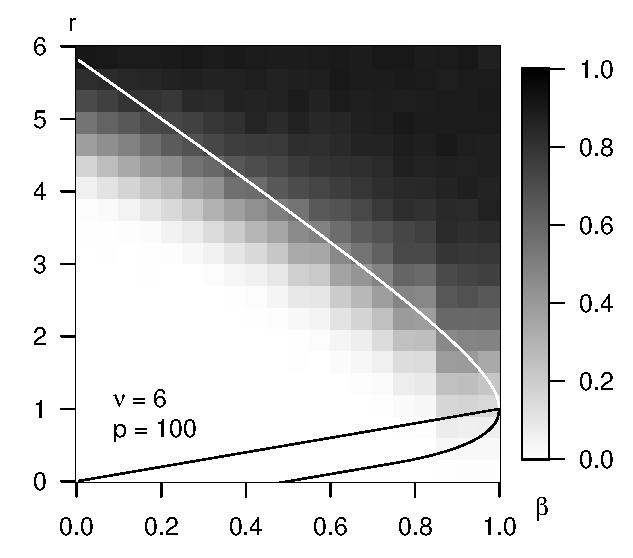
\includegraphics[width=0.4\textwidth]{./simulated_phase_diagram_chi-squared_nu6_p100.eps}
      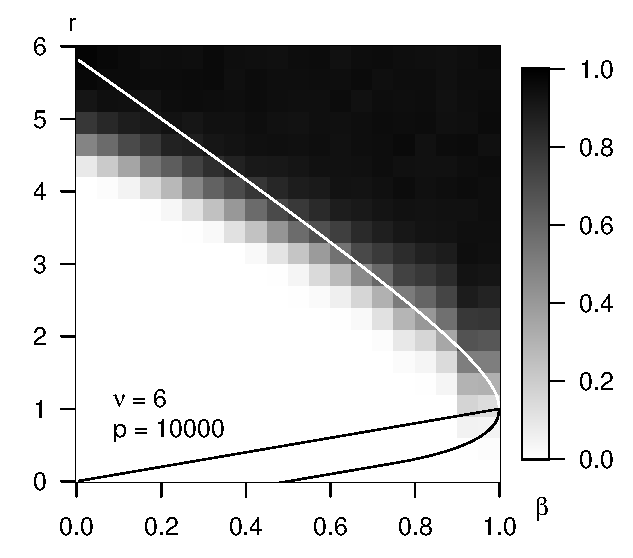
\includegraphics[width=0.4\textwidth]{./simulated_phase_diagram_chi-squared_nu6_p10000.eps}
      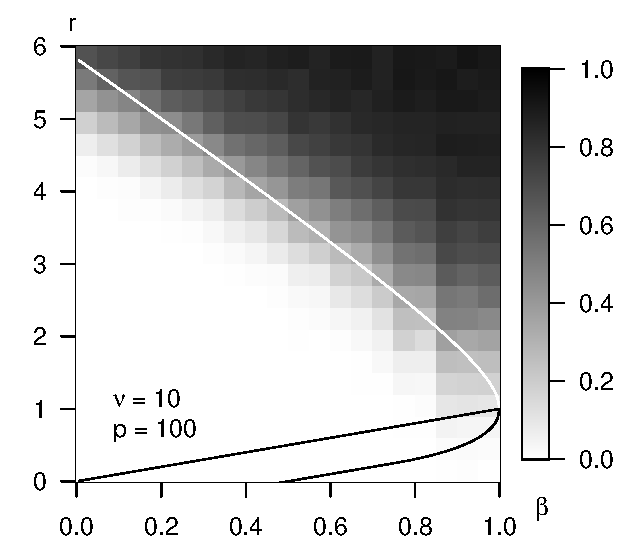
\includegraphics[width=0.4\textwidth]{./simulated_phase_diagram_chi-squared_nu10_p100.eps}
      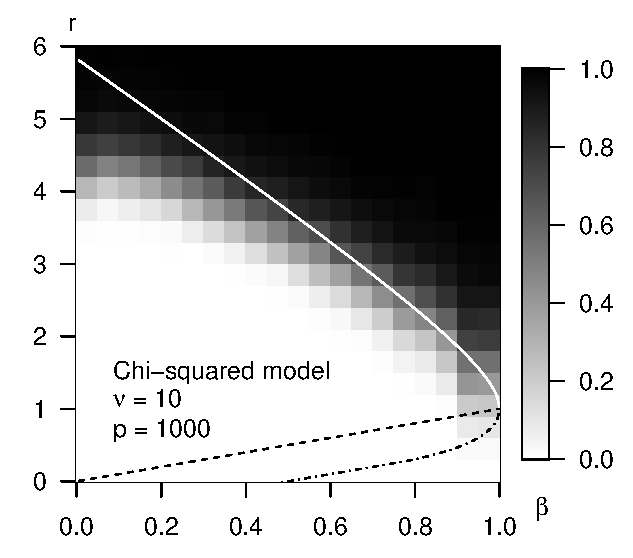
\includegraphics[width=0.4\textwidth]{./simulated_phase_diagram_chi-squared_nu10_p10000.eps}
      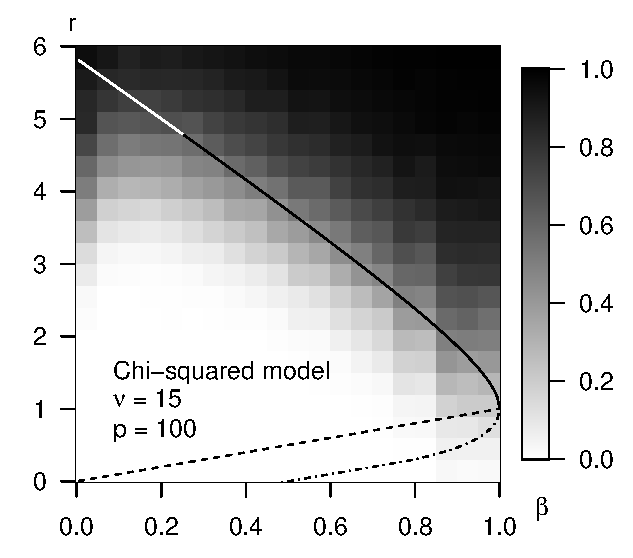
\includegraphics[width=0.4\textwidth]{./simulated_phase_diagram_chi-squared_nu15_p100.eps}
      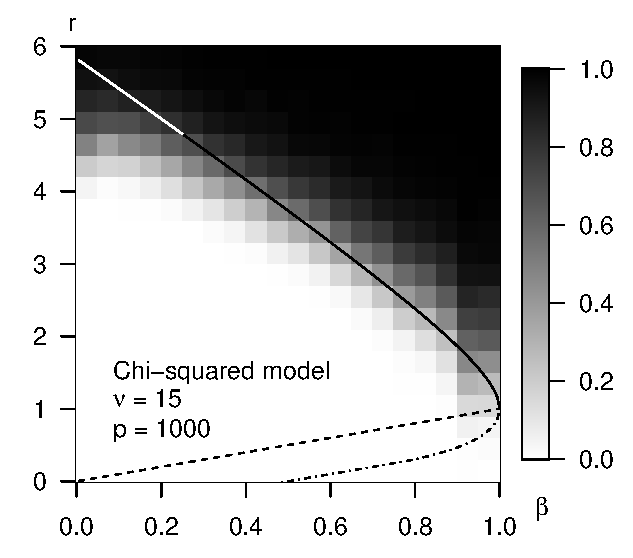
\includegraphics[width=0.4\textwidth]{./simulated_phase_diagram_chi-squared_nu15_p10000.eps}
      % 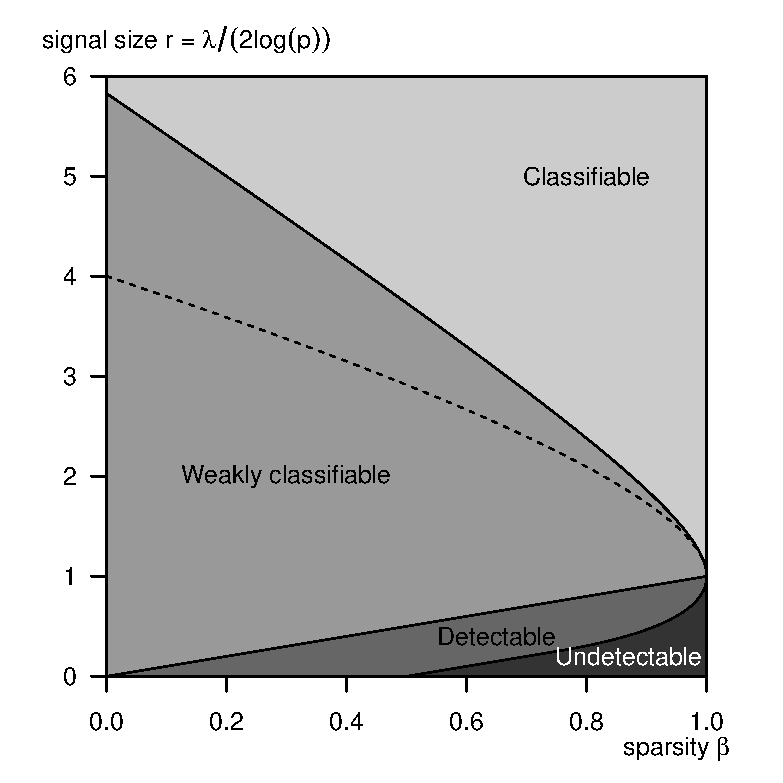
\includegraphics[width=0.35\textwidth]{./phase_diagram_chisquared.eps}
      \caption{The empirical probability of exact support recovery with oracle procedures in the Chi-squared model \eqref{eq:model-chisq}. 
      We simulate $\nu=6$ (upper), $\nu=10$ (middle), and $\nu=15$ (lower), for dimensions $p=100$ (left) and $p=10000$ (right), for an array of sparsity levels $\beta$ and signal sizes $r$.
      The experiments were repeated 1000 times for each sparsity-signal size combination; darker color indicates higher probability of exact support recovery.  
      Numerical results agree with the boundaries described in Theorem \ref{thm:chi-squred-strong-boundary}; the boundaries are largely unaffected by degrees of freedom.
      There are noticeable artifacts near $\beta=0$ in finite dimensions for oracle procedures. 
      The dash lines represent the weak classification boundary in Theorem \ref{thm:chi-squred-weak-boundary}, and the dash-dotted lines represent the detection boundary (see \citep{donoho2004higher}).} 
      \label{fig:phase-simulated-chi-squared}
\end{figure}



\subsection{The weak classification boundary in finite dimensions}


\subsection{Phase transitions of reported findings from GWAS}